%% This document gives an example on how to use the gucmasterthesis
%% LaTeX document class.
%% Use oneside for PDF delivery and twoside for printing in a book style
%% use language english or norsk and one of the following shortenings
%%  ``BSP'' Bachelor i Spillprogrammering,\\
%%  ``BRD'' Bachelor i drift av nettverk og datasystemer,\\
%%  ``BIS'' Bachelor i Informasjonssikkerhet,\\
%%  ``BPU'' Bachelor i Programvareutvikling, \\
%%  ``BIND'' Bachelor i Ingeni�rfad - data. 
\documentclass[BIS,english,oneside]{gucthesis}


\usepackage[utf8]{inputenc}     % For utf8 encoded .tex files
\usepackage[pdftex]{graphicx, hyperref}   % For cross references in pdf
\usepackage{color}              % For colouring text   
\usepackage{usecases}

\newcommand{\comment}[1]{\textcolor{blue}{\emph{#1}}}  %% use of the colour and you can see how to use commands with parts \comment{so what}

%% The class files defines these two
%% \newcommand{\GUC}{{G}j\o{}vik {U}niversity {C}ollege} %the extra {'s protect upper case
%% \newcommand{\HiG}{{H}\o{}gskolen i {G}j\o{}vik}

% you can create you one #define like structures using the \newcommand feature
% you can change behaviour using \renewcommand

\newcommand{\com}[1]{{\color{red}#1}} % supervisor comment
%\renewcommand{\com}[1]{} %remove starting % to remove supervisor comments

\newcommand{\todo}[1]{{\color{green}#1}} % items to do
%\renewcommand{\todo}[1]{} %remove starting % to remove items to do

\newcommand{\n}[1]{{\color{blue}#1}} % other comment
%\renewcommand{\n}[1]{} %remove starting % to remove notes

\newcommand{\dn}[1]{} % add the d to a note to say that you have finished with it.


% Norwegian Characters,  needs the {} or to be separate from the next letters
% \o{}   \aa{}   \ae{}   so at the end of a word you can use \o  \aa   \ae
% \O{}   \AA{}   \AE{}   you can also just leave a space and latex will remove it
%                        eg,  H\o gskolen i Gj\o vik


\begin{document}

\thesistitle{Snort Rule Manager}
\thesisauthor{Thomas Nyheim}
\thesisauthorA{Eirik Skogstad}
\thesisauthorB{Eigil Obrestad}
\thesissupervisor{Slobodan Petrovic}

\gmtkeywords{Thesis, Latex, Template, IMT}
\gmtdesc{This is the short description of a bachelor thesis}
\gmtnumber{-} % this is the number given to your project. May not be used  

\gmtoppdragsgiver{H\o gskolen i Gj\o{}vik}
\gmtcontact{Erik Helm\aa s, erik.helmas@hig.no, 61135000}




\thesisdate{\gucthesisdate}
\useyear{25.05.2014}

\gmtappnumber{} %numebr of appendixes
\gmtpagecount{} %currently auto calculated but might be wrong


\thesistitleNOR{Snort Rule Manager}
\gmtkeywordsNOR{Norway, Norsk}
\gmtdescNOR{This should be in Norwegian, I thought I would add some more text
to make sure that it ran over multiple lines. I will need to check the page
number feild as it probably should be just the core pages without the
appendices.  Currently it returns the last page of the whole document. 
If I cannot work it out, I will provide two inputs, gmtnumberpages and gmtappnumber.
That should do the job.}

 % this is the file which contains all the details about your thesis

\makefrontpages % make the frontpages

%pick the file you need from one of these two.
%\input{mastersIntro}
\chapter*{Preface} %the * means do not give the chapter a number
\label{chap:preface}

We would like to thank Erik Hjelm\aa{}s for motivating the development of a \Latex{} template
 for GUC's master's theses.  This has expanded to include Bachelor and perhaps soon the PhD 
 template.
 
 




\tableofcontents
\listoffigures
\listoftables


\chapter{Introduction}
\label{chap:introduction}

Starting in 2005, \GUC (GUC) was given the
right to issue Master diplomas. As a consequence of this, directions
for the master's thesis have been developed~\cite{GUCMaster},
including guidelines for the typographical details. These detailed
typographical rules have been implemented in the
\texttt{gucmasterthesis} \LaTeX\ document class.

The purpose of this document is to provide an example and description
on how this class file can be used.

This was then extended to include bachelor project by Simon McCallum.
The package has changed names and version number it is now called
\texttt{gucthesis}
v\gucthesisversion\ as of \gucthesisdate.


\chapter{Packages}
\label{chap:packages}

The \texttt{gucthesis} is built upon the standard \LaTeX\
\texttt{report} class. All commands from the \texttt{report} class can
be used, with the two exceptions of \verb+\subsubsection+ and
\verb+\paragraph+. This is because there should only be three
levels of headings according to the guidelines~\cite{GUCMaster}.

\section{Packages Used by gucthesis}
\label{sec:packages}

In addition to the \texttt{report} document class,
\texttt{gucthesis} makes direct use of the following packages
that must hence be present:
\begin{description}
	\item[geometry:] used for setting the sizes of the margins and
  	headers.
	\item[fontenc:] used with option \texttt{T1} for forcing the Cork font
  	encoding (necessary for the Charter font).
	\item[charter:] load Charter as the default font.
	\item[euler:] load the Euler math fonts.
	\item[babel:] to load language specific strings. Reasonable options
	  include \texttt{british}, \texttt{american}, \texttt{norsk},
	  \texttt{nynorsk} and \texttt{samin}.
\end{description}

\section{Other Relevant Packages}
\label{sec:otherpackages}

The author of a thesis might want to use a bunch of different packages
to those described in Section~\ref{sec:packages} in order to have all features needed for their document. 
In particular, it is advised to use the following:
\begin{description}
	\item[inputenc:] to allow \LaTeX\ to use more than 7-bit ASCII for its
	  input. Most often, the option \texttt{latin1} will do.
	\item[graphicx:] to include graphics.
	\item[hyperref:] this is a very nice package that makes cross links in
	  pdf documents. Use with option \texttt{dvips} or \texttt{pdftex}
	  in accordance with the driver that you use. Unfortunately, hyperref
	  is not completely bugfree\dots
\end{description}

\chapter{Structural Elements}
\label{chap:structural}

The title of the thesis should be set using the \verb+\thesistitle+
command, and the date of the thesis should be set using the
\verb+\thesisdate+ command. This makes the title and date appear in
the running header, like in this document.

\section{Page Layout}

The geometry of the page has been set using the \verb+\geometry+
command.

\section{Fonts}

Due to limited \LaTeX\ support for the Georgia font, Charter has been
chosen instead. For mathematical formula, the Euler fonts are used,
since they blend more nicely with the Charter than the standard
\LaTeX\ fonts: 
$$
 f(x) = \int_0^x g(\tau)\,d\tau
$$

For inline math you can use $\backslash{}($ and $\backslash{})$ for example \( f(x)= \frac{x^2}{1+x^2} \).  
This also allows you to use $\slash$ and $\backslash$. You need to include the \{\} when you want the special
character to have other letters immediately after it.

\section{Sectioning Commands}

The standard \LaTeX\ sectioning commands are used for both numbered
and unnumbered sections. The top level is given by the \verb+\chapter+
command. This starts a new right page. The two lower levels are
obtained using the \verb+\section+ and \verb+\subsection+ commands.
The standard \LaTeX\ \verb+\subsubsection+ and \verb+\paragraph+
commands have been disabled since their use is not encouraged by the
thesis guidelines. When you use these they will not be given numbers.  
They still appear in the document with highlighting but not in the 
table of contents.

\subsection{The subsection}

This is an example of a subsection.

\subsubsection{The subsubsection}

This is an example of a subsubsection.

\paragraph{The paragraph}

This is an example of a paragraph with a heading.

\section{Floats (Figures and Tables)}
\label{sec:floats}

Figures are placed in the \texttt{figure} environment. An example is
shown in Figure~\ref{fig:example}. %notice the ~ in between figure and the \ref. it stops latex from splitting the number and word over a line.
Tables are placed in the \texttt{table} environment. An example is given in
Table~\ref{tab:example}. Figures and tables float freely around in the
document in accordance with standard \LaTeX\ behavior.

\begin{figure}[tbp]  %t top, b bottom, p page | you can also use h to try to get the figure to appear at the current location
  \centering
  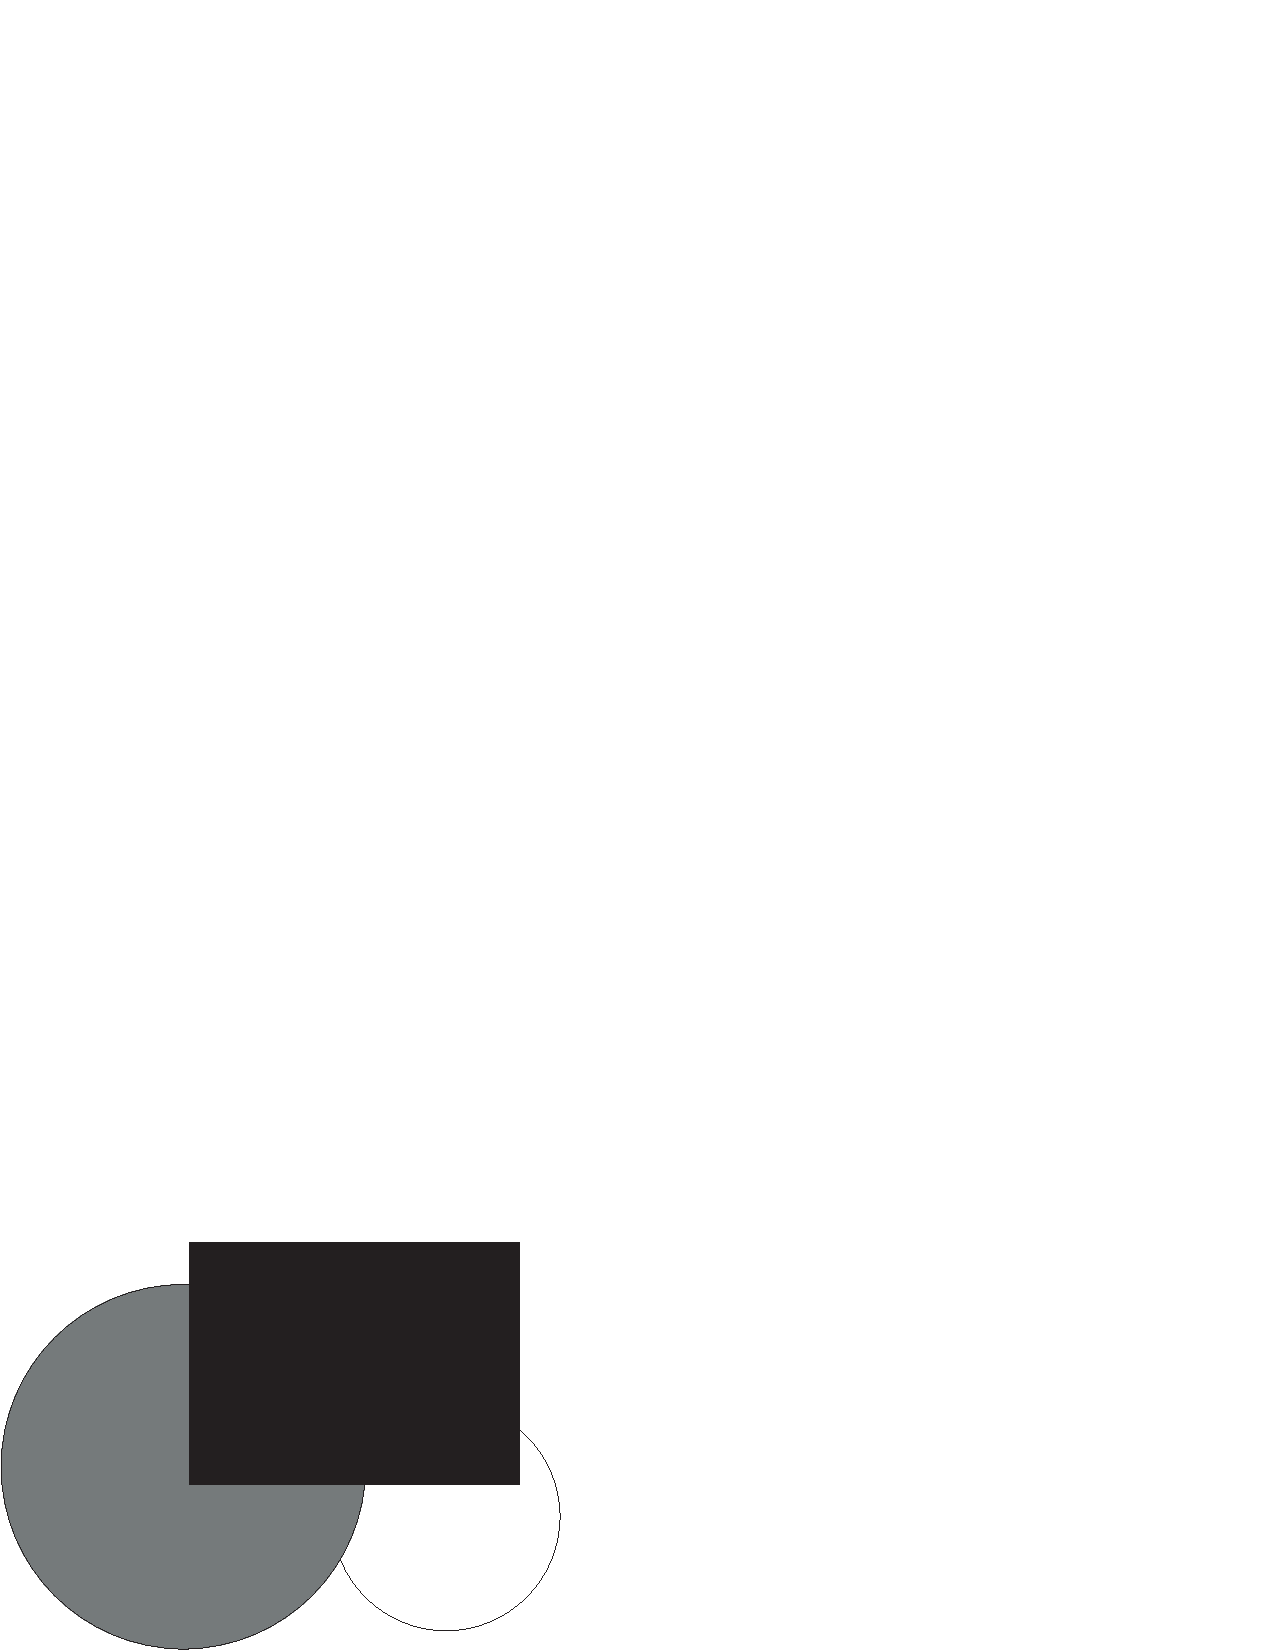
\includegraphics[width=.5\textwidth]{example_fig}
  \caption[An example figure.]{An example figure. If the caption is
    shorter than one line, it is centered. If it goes over more than
    one line, it is left and right justified. Furthermore, it is
    suggested that an alternative short caption is given in order to
    produce a good list of figures.}
  \label{fig:example}
\end{figure}

\begin{table}[tbp]
  \centering
  \begin{tabular}{c|c}
    Age  & IQ  \\ 
    \hline
    10   & 100 \\
    20   & 100 \\
    30   & 150 \\
    40   & 100 \\
    50   & 100
  \end{tabular}
  \caption{An example table.}
  \label{tab:example}
\end{table}

The captions are placed \emph{below} both for the figures and the
tables. The caption is set in 9pt. If the caption is shorter than one
line, it is centered.

\section{Quotes}
\label{sec:Quotes} % this allows you to refer to this section number using \ref{sec:Quotes}

Quotes are inserted using the standard \LaTeX\ \texttt{quote}
environment. The environment has been changed so that a 9pt font is
used:

\begin{quote}
  ``And I looked, and, behold, a whirlwind came out of the north, a
  great cloud, and a fire infolding itself, and a brightness was about
  it, and out of the midst thereof as the colour of amber, out of the
  midst of the fire. Also out of the midst thereof came the likeness
  of four living creatures.''
\end{quote}

\section{Lists}
\label{sec:lists}

Point lists and enumerated lists are made by using the standard
\texttt{itemize} and \texttt{enumerate} environments, respectively.
The spacing is going to be changed in accordance with the specification. For
\texttt{itemize}, the results look like this:
\begin{itemize}
	\item First item.
	\item Second item. Here I will put some long text, just to illustrate.
	  Here I will put some long text, just to illustrate. Here I will put
	  some long text, just to illustrate. Here I will put some long text,
	  just to illustrate.
	\item Third item also has subitems:
	  \begin{itemize}
		  \item First subitem.
		  \item Second subitem.
		  \item Third subitem.
	  \end{itemize}
\end{itemize}
and for \texttt{enumerate} like this:
\begin{enumerate}
	\item First item.
	\item Second item. Here I will put some long text, just to illustrate.
	  Here I will put some long text, just to illustrate. Here I will put
	  some long text, just to illustrate. Here I will put some long text,
	  just to illustrate.
	\item Third item also has subitems:
	  \begin{enumerate}
		  \item First subitem.
		  \item Second subitem.
		  \item Third subitem.
	  \end{enumerate}
\end{enumerate}

You may also want to use descriptive lists
\begin{description}
	\item[First] the first item.
	\item[Second] the second item. Here I will put some long text, just to illustrate.
	  Here I will put some long text, just to illustrate. Here I will put
	  some long text, just to illustrate. Here I will put some long text,
	  just to illustrate.
	\item [What now] the third item also has subitems:
	  \begin{enumerate}
		  \item First subitem.
		  \item Second subitem.
		  \item Third subitem.
	  \end{enumerate}
\end{description}


\section{Bibliographic References}

You should cite articles~\cite{Askvall1985}, books~\cite{Card1983},
anthologies~\cite{Lancaster1985} and web publications~\cite{Meldon1997}
like this. There is always an issue referencing web pages. Currently
we suggest that you use the HiG Website~\cite{HiG:Website}.


A particular bibliography style file for GUC named
\texttt{gucthesis.bst} has been developed based upon the
standard Bib\TeX\ \texttt{unsrt} style.


%%This is a very basic article template.
%%There is just one section and two subsections.
\documentclass{article}
\usepackage{usecases}
\usepackage{fullpage}

\begin{document}

\section{High-level use cases}

\begin{usecase}
\addtitle{Use case}{Manual rule update}
\addfield{Primary actor}{User}
\addfield{Purpose}{Update the central rule database}
\addfield{Description}{The user sends a command to trigger a rule update, and
the system pulls rule files from all the sources specified in the list of
sources. Rules are then processed and stored in the database.}
\addfield{Preconditions}{One or more sources must exist}
\addfield{Postconditions}{The central rule database is up to date with the
newest rules from all sources}
\end{usecase}

\begin{usecase}
\addtitle{Use case}{Automatic rule update}
\addfield{Primary actor}{System}
\addfield{Purpose}{Update the central rule database}
\addfield{Description}{At configured time-intervals, the system is triggered to
update and pulls rule files from all the sources specified in the list of sources, processes the rules and then stores them in the database.}
\addfield{Preconditions}{One or more sources must exist}
\addfield{Postconditions}{The central rule database is up to date with the
newest rules from all sources}
\end{usecase}

\begin{usecase}
	\addtitle{Use case}{Treshold is applied/removed to rule}
	\addfield{Description}{User sends a command with either tresholding parameters or removal of threshold for a rule and the system updates the database to reflect the change. One threshold parameter per rule.}
\end{usecase}

\begin{usecase}
	\addtitle{Use case}{Suppression is applied to rule}
	\addfield{Description}{User sends a command with either suppression parameters or removal of threshold for a rule and the system updates the database to reflect the change. Suppression parameters can take multiple IP-addresses/IP-ranges.}
\end{usecase}

\begin{usecase}
	\addtitle{Use case}{Viewing rules}
	\addfield{Description}{Rules are retrieved from the database, processed for GUI/CLI format and then delivered to GUI or CLI in specified format.}
\end{usecase}

\begin{usecase}
	\addtitle{Use case}{User comments on rule or rule set}
	\addfield{Description}{User specifies a rule or rule set and applies a comment to it, that is then stored in the database.}
\end{usecase}

\begin{usecase}
	\addtitle{Use case}{User edits/deletes a comment on a rule or rule set}
	\addfield{Description}{User specifies a rule or rule set and edits or deletes it from the database.}
\end{usecase}

\begin{usecase}
	\addtitle{Use case}{User registers a sensor}
	\addfield{Description}{User sends parameters for a sensor and the system stores the parameters in the database. }
\end{usecase}

\begin{usecase}
	\addtitle{Use case}{User registers a source for rule updates}
	\addfield{Description}{User sets parameters for sources and the system stores the parameters in the database.}
\end{usecase}

\begin{usecase}
	\addtitle{Use case}{System verifies rules as valid and functional}
	\addfield{Description}{Before rules are stored in the database, the system process and check them for validity and functionality by doing a test run in a local SNORT to catch any errors they might produce and register in the database }
\end{usecase}

\begin{usecase}
	\addtitle{Use case}{User organizes sensors into sensor group}
	\addfield{Description}{A user sets up a sensor group and then includes one or more sensors into this group. The user can then manipulate rules on a sensor group basis.}
\end{usecase}

\begin{usecase}
	\addtitle{Use case}{Rules are distributed by the user}
	\addfield{Description}{User sends a command to distribute to specified sensors and the system retrieves rule information for the database, processes them and formats them for SNORT, then distributes them to all sensors specified per their individual settings.}
\end{usecase}

\begin{usecase}
	\addtitle{Use case}{Rules are distributed by the system}
	\addfield{Description}{Configured at intervals, the system triggers a command to distribute to specified sensors and the system retrieves rule information for the database, processes them and formats them for SNORT, then distributes them to all sensors specified per their individual settings.}
\end{usecase}

\section{Detailed use cases}

\begin{usecase}
	\addtitle{Use case}{Central rule database update}
	\addfield{Primary actor}{System}
	\addfield{Purpose}{Update the central rule database from external sources}
	\addfield{Description}{
		\begin{enumerate}
		  \item The case is triggered when either the user issues the command to
		  update, or the system (daemon) issues the command based on a set time-interval. The user has the option to update rules from a local file, if this is the case, the program will proceed from part 3.
		
		\item The process starts in the Rule Downloading Module where each rule source is
	checked for updates by comparing MD5 values. If the MD5 values differ, the module will  retrieve the updated rule files and pass them along to the Rule Pre-Storage Processing Module. 
		
		\item The Rule Pre-Storage Processing Module then begins reading the files line
	by line and parses metadata from the new rule files. The rules are checked against the current rules stored in the database to identify which rules are new or modified. Based on this identification, the new or modified rules are parsed into complete objects and passed to the Database/Core Module that stores the new or modified rules into the database.
	One or more rule sources must be registered in the system. Alternatively, one or more local rule files must be present.
	Rules have either been confirmed as up-to-date or the new or updated rule objects have been passed to the Database Module. 
		\end{enumerate}
	}
	\addfield{Preconditions}{}
	\addfield{Postconditions}{}
	\addfield{Triggers}{
		Manual rule update,
		Automatic rule update
	}
	\addscenario{Basic Flow:}{
		\item Update is triggered
		\item Rule Downloading Module compares source with stored rules.
		\item Updated rule files are downloaded from sources. The files are validated
		and passed to the Pre-Storage Processing Module module.
		\item The new files are parsed for rule SID and revision number. 
		\item A list of rule SID and revision numbers are gathered from the database
		and these are compared to identify which rules are new or modified.
		\item New or changed rules are then parsed completely into full objects and
		these objects are passed to the Database/Core Module.
		\item The Database/Core Module stores the new or changed rule objects into the
		database.
	}
	\addscenario{Extensions:}{
		\item 
		\begin{enumerate}
			\item Update is triggered by user
			\item Update is triggered by system
		\end{enumerate}
		\item 
		\begin{enumerate}
			\item The rules at source is equal to the stored rules. Database is up to date, so no more action is required. 
			\item The rules at source is newer than stored rules. Database must be updated.
		\end{enumerate}
		\item
		\begin{enumerate}
			\item User is notified that database is up to date. 
			\item User is notified that the database is not up to date and an update process has begun.
		\end{enumerate}
		\setcounter{enumi}{8}
		\item
		\begin{enumerate}
			\item The user is notified that the update is complete. 
			\item The user is notified that rules have been updated during since the last scheduled update interval.
		\end{enumerate}
		
	 }
	\addscenario{Error handling:}{
		\item The source and database checksum is different but the source rules are
		older than what is stored in the database: \textit{The program can still
		continue, because if the SIDs already exist they will not be added again and if the revisions are older the rules will also not be updated.}
		\item A ruleset has changed its name or one or more rules are moved to a
		different ruleset: \textit{Based on a configuration file, the affected rules
		will either be a) automatically moved to the new ruleset or b) stay put in their
		original ruleset. The user will be notified and can choose to reverse or
		distribute the changes.}
		}
\end{usecase}

\begin{usecase}
	\addtitle{Use case}{Globally enable/disable a rule or ruleset}
	\addfield{Primary actor}{User}
	\addfield{Purpose}{Turn a rule or ruleset on/off}
	\addfield{Description}{User sends a command to enable/disable a specified
	rule or ruleset, and the system updates the database to reflect that the rule
	is enable/disabled.}
	\addfield{Preconditions}{The rule or ruleset must exist in the database}
	\addfield{Postconditions}{The rule or ruleset is deativated on all sensors
	\textbf{except} if this setting is overridden in a sensor's local
	RuleModifier.}
\end{usecase}


\begin{usecase}
	\addtitle{Use case}{Locally enable/disable a rule or ruleset on a sensor}
	\addfield{Primary actor}{User}
	\addfield{Purpose}{Turn a rule or ruleset on/off on a sensor}
	\addfield{Description}{A user wants to either enable or disable a rule or rule
	set on one or more sensors. This is done by sending a command that specifies
	which rule or rule set is to be affected, how it is affected and on which
	sensor or sensors are affected. The central database must be updated with this
	new status and the change must be pushed out to the affected sensor or sensors.}
	\addfield{Preconditions}{One or more rule sets or rules must be present in the central database. One or more sensor must be registered.}
	\addfield{Postconditions}{The changes to the rule or rule set must be reflected on the affected sensor or sensors.}
	\addfield{Triggers}{}
	\addscenario{Basic flow}{
		\item The user enables/disables a rule on a given sensor.
		\item The central database changes the status of the rule or rule set by
		manipulating the status flags.
		\item The system notifies the sensor that a change has occurred. 
		\item The change is synced to the affected sensor. 
	}
	\addscenario{Error handling:}{
		\setcounter{enumi}{3}
		\item The change may never be synced to the sensor due to errors: \textit{There must be an error protocol that is followed in this scenario.}
		} 
\end{usecase}

\begin{usecase}
	\addtitle{Use case}{Rule is modified/de-modified with a threshold or suppression on one or more sensors}
	\addfield{Primary actor}{User, System}
	\addfield{Purpose}{Manipulate configurations for specific rules on specific sensors.}
	\addfield{Description}{A user wants to either turn on or off a threshold or suppression modifier on a rule on one or more sensors. This is done by sending a command that specifies which rule the modification will apply to, the parameters of the modification and for which sensor or sensors this will apply for. The central database must be updated with this new status and the change must be pushed out to the affected sensor or sensors.}
	\addfield{Preconditions}{One or more rule sets or rules must be present in the central database. One or more sensors must be registered.  If a modification is applied, there must not be another modification for the same rule on the same sensor. If a modification is removed, it must already exist.}
	\addfield{Postconditions}{The modifications must be applied on the rule and sensor or sensors in question.}
	\addfield{Triggers}{}
	\addscenario{Basic flow}{
		\item User sets a threshold/suppression on a rule on a sensor.
		\item The central database creates a threshold/suppression for the specified rule and the specified sensor.
		\item The system notifies the sensor that a change has occurred.
		\item The change is synchronized to the affected sensor.
	}
	\addscenario{Extensions}{
		\item User turns off a threshold/suppression on a rule on a sensor
		\item The central database deletes the threshold/suppression for the specified rule and the specified sensor.
	}
	\addscenario{Error handling}{
		\item The change may never be synced to the sensor due to errors: \textit{There must be an error protocol that is followed in this scenario.}
	}
\end{usecase}

\begin{usecase}
	\addtitle{Use case}{Rules are distributed}
	\addfield{Primary actor}{User, System, Sensor}
	\addfield{Purpose}{Distribute rules from the central database to the local
	sensors}
	\addfield{Description}{A user or the system wants to synchronize the rules
	stored in the central database to either one, multiple or all sensors. This is initiated either by the user sending a command or by the system having a regular interval. The system must then calculate and organize the central database data so that the affected sensors get synchronized.}
	\addfield{Preconditions}{One or more rule sets or rules must be present in the
	central database. One or more sensors must be registered}
	\addfield{Postconditions}{The rules on a local sensor must be in sync with the
	central database.}
	\addfield{Triggers}{}
	\addscenario{Basic flow}{
		\item Synchronize signal is sent.
		\item The system calculates and organizes the data for each sensor affected by the synchronization.	
		\item The system initializes a synchronization protocol with the affected sensor or sensors, sending a list of what the sensor should have.	
		\item The sensor calculates diff between should have and has.
		\item Compare diff.
		\item Send update.
		\item The sensor includes the new changes into its database and files. Tells the central system that it is now up to date.
		\item The system carries out maintenance to reflect the synchronization.
		\item The user is notified that all sensors affected are now up to date.			
	}
	\addscenario{Extensions}{
		\item
		\begin{enumerate}
			\item User sends a command to synchronize one, more or all sensors		
			\item The system reaches an interval for synchronizing all sensors.		
		\end{enumerate}
		\etcounter{enumi}{4}
		\item
		\begin{enumerate}
			\item The sensor content is different from what it should have, asks central system to send what it needs.
			\item The sensor content is not different from what it should have, no further action is required. This status is sent to the central system.
		\end{enumerate}	
		\item
		\begin{enumerate}
			\item The system retrieves and sends what the sensor asks for.
			\item The system terminates the synchronization protocol with the sensor in question.
		\end{enumerate}				
	}
	\addscenario{Error handling}{
	1. The change may never be synced to the sensor due to errors. Solution: There
	must be an error protocol that is followed in this scenario.
	}
\end{usecase}



\end{document}

\bibliographystyle{gucthesis}
\bibliography{SRM_references}

\appendix %after this line all chapters will have leters instead of numbers

\chapter{Meetings}

You can include an Appendix of the log of your meeting for example


\end{document}